% Provenance (never printed): old terminale S material on magmatism in
% subduction zones (volcanic arcs above the slab, water released by the slab
% and hydrous melting of the mantle wedge, andesitic volcanism and granitoid
% plutons, growth of the continental crust). Owner (Sync 0): volcanic arc,
% hydrous melting, granodiorite, batholith, continental growth. Subduction,
% slab, Wadati-Benioff zone, blueschist and eclogite are g11.06's; partial and
% decompression melting and peridotite g11.05's; andesite, diorite, rhyolite,
% pluton g11.08's; continental crust g12.01's; magma, explosive eruption Book 1's
% (g7): recalled, never redefined. Figures: figdata/grade-12/arc_magmatism.py
% (GVP volcanoes, ComCat NE Japan band, dry solidus via grade-11
% geotherm_solidus.py, wet solidus brackets of Wang 2020 and Kawamoto-Holloway 1997).
\chapter{Magmatisme bij subductiezones}\label{ch:g12:subduction-magmatism}

Op 18 mei 1980, om 8.32 uur 's ochtends, schudde een aardbeving met magnitude 5.1
de Mount St.~Helens door elkaar. Meteen gleed de noordflank van de vulkaan, die
al ongeveer twee meter per dag naar buiten opbolde, weg: de grootste
puinlawine in de geschreven geschiedenis, ongeveer \qty{2.5}{km^3} gesteente. Bevrijd van zijn
last blies het gasrijke magma binnenin zijdelings naar buiten door het litteken, met minstens
\qty{480}{km/h}, en het maaide bossen plat over \qty{600}{km^2}. Binnen
vijftien minuten stond er een aszuil van meer dan \qty{24}{km} hoog, en de
uitbarsting duurde negen uur. Eenenzestig mensen kwamen om of werden nooit gevonden.
% ledger: usgs:b2-msh-1980, usgs:msh-deaths

\begin{omfigure}
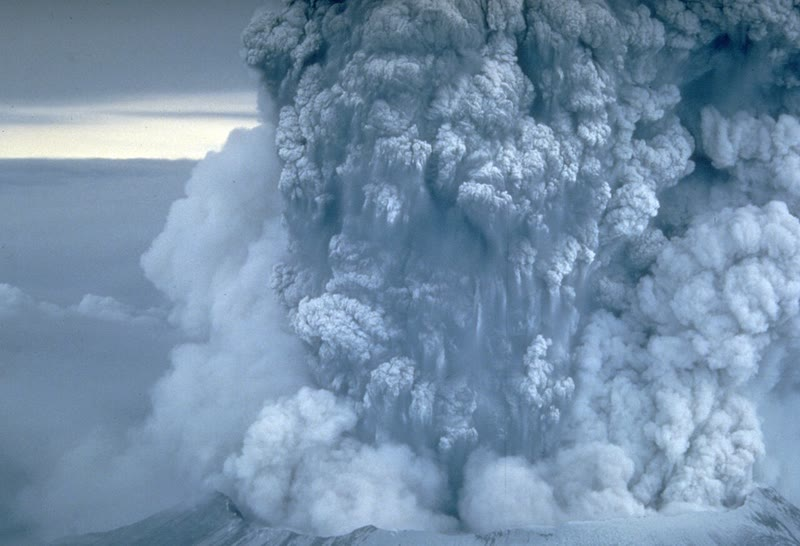
\includegraphics[width=0.55\linewidth]{images/book2/g12-swanson-st-helens-plume.jpg}

{\small De aszuil van de Mount St.~Helens op 18 mei 1980, die in minder dan vijftien
minuten meer dan \qty{24}{km} hoog werd. Foto Donald
A.~Swanson, USGS (publiek domein).}
\end{omfigure}
% ledger: photo:g12-st-helens, usgs:b2-msh-1980

De Mount St.~Helens is een van een rij vulkanen --- Baker, Rainier, Hood,
Shasta en andere --- die boven de plaats staat waar een kleine oceanische
plaat, de Juan de Fucaplaat, onder Noord-Amerika zinkt. Dit hoofdstuk
vraagt waarom daar vulkanen te vinden zijn, waarom hun uitbarstingen zo vaak heftig zijn,
en wat er wordt van het magma dat het oppervlak nooit bereikt.
% ledger: earle:cascades

\begin{recall}
Bij een \omterm{def:g11:subduction-zones:subduction}{subductiezone} zinkt een plaat \omterm{def:g11:ocean-ridges:oceanic-lithosphere}{oceanische lithosfeer} terug in de
mantel onder een andere plaat; haar aardbevingen, de \omterm{def:g11:subduction-zones:benioff}{Wadati--Benioffzone},
volgen de \omterm{def:g11:subduction-zones:slab}{slab} tot op wel \qty{670}{km} diepte
(\cref{ch:g11:subduction-zones}). De mantel bestaat uit \omterm{def:g11:ocean-ridges:peridotite}{peridotiet}; hij is
vast, maar een gesteente dat opstijgt en minder wordt samengedrukt, kan gedeeltelijk smelten, door
\omterm{def:g11:ocean-ridges:partial-melting}{decompressiesmelten}, zoals onder een rug (\cref{ch:g11:ocean-ridges}).
\omterm{def:g11:igneous-rocks:rock-names}{Andesiet} is een \omterm{def:g11:igneous-rocks:volcanic-plutonic}{vulkanisch gesteente} tussen basalt en \omterm{def:g11:igneous-rocks:rock-names}{ryoliet}, \omterm{def:g11:igneous-rocks:rock-names}{dioriet} zijn plutonische
tegenhanger, en een \omterm{def:g11:igneous-rocks:intrusion}{pluton} een groot magmalichaam dat ondergronds is afgekoeld
(\cref{ch:g11:igneous-rocks}). De \omterm{def:g12:continental-crust:continental-crust}{continentale korst} is dik en licht,
bovenaan vooral granitisch gesteente (\cref{ch:g12:continental-crust}). Een explosieve
uitbarsting blaast het magma met zijn eigen gas aan stukken (Boek 1, jaar 7).
\end{recall}
% ledger: tulane:magma-types, tulane:intrusions, rg14:crust

\section{Vulkanische bogen}

De meeste actieve vulkanen op het land staan niet zomaar ergens. Van de 1214
vulkanen die sinds het einde van de laatste ijstijd zijn uitgebarsten en die zijn opgenomen
in de catalogus van het Global Volcanism Program, staan er 838 --- meer dan twee op de
drie --- boven een \omterm{def:g11:subduction-zones:subduction}{subductiezone}. Rond de Stille Oceaan vormen ze een
bijna ononderbroken ring, vaak de Ring van Vuur genoemd, en elke rij ervan
loopt evenwijdig aan een trog, aan de kant van de plaat die niet zinkt.
% values: n_volcanoes 1214, n_subduction 838, frac_subduction 0.690 (arc_magmatism.py)
% ledger: data:gvp, tulane:arc

\begin{omfigure}
\begin{tikzpicture}
\begin{axis}[ommap, width=\linewidth, xtick={-180,-90,...,180}, ytick={-60,0,60},
  legend style={font=\scriptsize, at={(0.5,-0.13)}, anchor=north, legend columns=3,
    /tikz/every even column/.append style={column sep=6pt}}]
\addplot[fill=omLithAlluv, draw=black!45, line width=0.2pt, forget plot] table {figdata/out/shared-geo-land.dat};
\addplot[black!70, line width=0.5pt, forget plot] table {figdata/out/shared-geo-school-subduction.dat};
\addplot[fill=black!70, draw=none, forget plot] table {figdata/out/shared-geo-school-teeth.dat};
% computed in figdata/grade-12/arc_magmatism.py; ledger: data:gvp, data:pb2002, data:ne-land
\addplot[only marks, mark=triangle*, mark size=1.1pt, black!40] table[x=lon, y=lat] {figdata/out/grade-12-arc_magmatism-world-other.dat};
\addplot[only marks, mark=triangle*, mark size=1.3pt, omThm] table[x=lon, y=lat] {figdata/out/grade-12-arc_magmatism-world-sub.dat};
\addlegendimage{black!70, line width=0.5pt}
\legend{{andere vulkanen}, {vulkanen boven een subductiezone}, {trog}}
\end{axis}
\end{tikzpicture}

{\small De vulkanen die sinds het einde van de laatste ijstijd actief zijn, rood waar
ze boven een \omterm{def:g11:subduction-zones:subduction}{subductiezone} staan, met de troggen (zwarte lijn, driehoekjes
op de plaat die erover schuift). Gegevens: Smithsonian Global Volcanism Program;
plaatgrenzen van Bird (2003); land van Natural Earth.}
\end{omfigure}
% values: n_subduction 838 of 1214 (arc_magmatism.py)

\begin{definition}[Vulkanische boog]\label{def:g12:subduction-magmatism:arc}
Een \emph{vulkanische boog}\index{vulkanische boog} is een rij vulkanen op de
bovenliggende plaat van een \omterm{def:g11:subduction-zones:subduction}{subductiezone}, evenwijdig aan de trog, die
staat boven de plaats waar de \omterm{def:g11:subduction-zones:slab}{slab} een diepte van ongeveer honderd
kilometer heeft bereikt. Het is een \emph{eilandboog} wanneer hij uit de zeebodem oprijst, zoals
in Japan of Indonesië, en een continentale boog wanneer hij op een continent staat,
zoals in de Andes of de Cascades.
\end{definition}
% ledger: tulane:arc, earle:arc-water, earle:cascades, sa06:slab-depth

De rand van de boog die het dichtst bij de trog ligt, heet het \textbf{vulkanische
front}: aan de trogkant ervan zijn er helemaal geen vulkanen. Hoe diep ligt
de \omterm{def:g11:subduction-zones:slab}{slab} eronder?

\begin{proposition}[De slab onder het vulkanische front]\label{prop:g12:subduction-magmatism:depth}
Als de \omterm{def:g11:subduction-zones:slab}{slab} een vlak is dat vanaf de trog onder een hoek $\theta$ helt, en
het vulkanische front op een horizontale afstand $d$ van de trog ligt, dan
ligt de bovenkant van de \omterm{def:g11:subduction-zones:slab}{slab} onder het front op een diepte
\[
  H = d \tan\theta .
\]
\end{proposition}

\begin{proof}
Neem een verticale doorsnede dwars op de trog. De \omterm{def:g11:subduction-zones:slab}{slab}, het oppervlak en de
verticale lijn onder het front vormen een rechthoekige driehoek, met de rechte hoek
onder het front: de zijde langs het oppervlak is $d$, de verticale zijde is
$H$, en de hoek bij de trog is $\theta$. Dus $\tan\theta = H/d$.
\end{proof}

Een overzicht van 839 vulkanische centra langs \qty{33000}{km} bogen mat
$H$ onder elk ervan: gemiddeld over stukken boog van \qty{500}{km} lang
loopt het van 72 tot \qty{173}{km}, met een gemiddelde van \qty{105}{km}. Bogen boven
steile \omterm{def:g11:subduction-zones:slab}{slabs} liggen dicht bij hun trog, bogen boven flauw hellende \omterm{def:g11:subduction-zones:slab}{slabs} ver
ervandaan, maar de \omterm{def:g11:subduction-zones:slab}{slab} eronder ligt altijd ongeveer honderd kilometer
diep.
% ledger: sa06:slab-depth

\begin{method}[De slab onder een vulkaan vinden]\label{met:g12:subduction-magmatism:slab}
\begin{enumerate}
  \item Neem de aardbevingen van een smalle band dwars over de boog, en zet hun
        diepte uit tegen hun afstand dwars over de boog, op ware schaal.
  \item Houd de aardbevingen dieper dan ongeveer \qty{70}{km}: ondiepere
        komen ook voor in de bovenliggende plaat en op de breuk tussen de twee
        platen.
  \item Trek de lijn, of lees de diepte af, van de diepe aardbevingen onder
        het vulkanische front: dat is daar de diepte van de \omterm{def:g11:subduction-zones:slab}{slab}.
  \item Controleer die met $H = d\tan\theta$, waarbij je $d$ vanaf de trog meet en
        de helling $\theta$ op de doorsnede.
\end{enumerate}
\end{method}

\begin{omfigure}
\begin{tikzpicture}
\begin{axis}[omsection, name=jp, scale only axis, width=0.8\linewidth, height=0.2857\linewidth,
  xmin=0, xmax=700, ymin=0, ymax=250, y dir=reverse,
  xlabel={afstand ten oosten van \ang{138}~OL (\unit{km})}, ylabel={diepte (\unit{km})},
  xtick={0,100,...,700}, ytick={0,50,...,250}, tick label style={font=\small},
  every axis label/.append style={font=\small}]
% computed in figdata/grade-12/arc_magmatism.py; ledger: data:b2-usgs-ne-japan, data:gvp, data:pb2002
\addplot[only marks, mark=*, mark size=0.55pt, black!35] table[x=x_km, y=depth] {figdata/out/grade-12-arc_magmatism-jp-quakes.dat};
\addplot[omDef, line width=0.9pt, dashed] table[x=x_km, y=depth] {figdata/out/grade-12-arc_magmatism-jp-slab.dat};
\addplot[only marks, mark=triangle*, mark size=2.6pt, omThm] table[x=x_km, y expr=-7] {figdata/out/grade-12-arc_magmatism-jp-volc.dat};
\draw[omThm, densely dotted, line width=0.8pt] (axis cs:259.2,0) -- (axis cs:259.2,98.2);
\fill[omThm] (axis cs:259.2,98.2) circle (1.6pt);
\coordinate (front) at (axis cs:259.2,-14);
\coordinate (trench) at (axis cs:528.9,-14);
\coordinate (H) at (axis cs:262,60);
\coordinate (slab) at (axis cs:95,228);
\draw[black, line width=0.9pt] (axis cs:528.9,-12) -- (axis cs:528.9,0);
\end{axis}
\node[font=\scriptsize, anchor=south, text=omThm] at (front) {vulkanisch front (Iwate)};
\node[font=\scriptsize, anchor=south] at (trench) {Japantrog};
\node[font=\scriptsize, anchor=west, text=omThm, fill=white, inner sep=1pt] at (H) {\qty{98}{km}};
\node[font=\scriptsize, anchor=west, text=omDef, fill=white, inner sep=1pt] at (slab) {slab, helling ongeveer \ang{20}};
\end{tikzpicture}

{\small Een doorsnede door het noordoosten van Japan op ware schaal: de aardbevingen met
magnitude 4.5 of meer tussen \ang{37.5} en \ang{40.5}~NB, 1976--2025 (grijs),
de vulkanen van dezelfde band (rode driehoekjes) en de lijn die is aangepast aan de
aardbevingen dieper dan \qty{70}{km} (blauw, gestreept). Twee op de vijf van de
ondiepe gebeurtenissen ten oosten van \ang{141.5}~OL dateren uit 2011, het jaar van de grote
aardbeving van maart. Gegevens: aardbevingscatalogus van de USGS;
Smithsonian Global Volcanism Program; plaatgrenzen
van Bird (2003).}
\end{omfigure}
% values: shallow (<70 km) events east of 141.5 E: 3622, of which 1451 in 2011 (0.40); ledger usgs:tohoku
% values: jp_front_lon 141.0 (x 259.2 km), jp_trench_lon 144.12 (x 528.9), jp_front_trench_km 269.4, jp_dip_deg 19.98, jp_H_geom 98.0, bin_141_median 98.15, jp_slab_depth_front 105.6 (arc_magmatism.py)

\begin{example}[Het noordoosten van Japan]\label{ex:g12:subduction-magmatism:japan}
In de band van de figuur is de oostelijkste vulkaan de Iwate, op \ang{141.0}~OL,
en de Japantrog ligt op \ang{144.1}~OL. Eén lengtegraad is daar
$111.2\cos\ang{39} \approx \qty{86.4}{km}$, dus $d \approx 3.12 \times 86.4
\approx \qty{270}{km}$. De diepe aardbevingen hellen ongeveer \ang{20}, en
\[
  H = 270 \times \tan\ang{20} \approx \qty{98}{km}.
\]
De aardbevingen dieper dan \qty{70}{km} die onder het front zelf liggen,
hebben een mediane diepte van \qty{98}{km}: de twee komen overeen, dicht bij het
wereldgemiddelde.
\end{example}
% values: km_per_deg_lon 86.415, jp_front_trench_km 269.4, jp_dip_deg 19.98, jp_H_geom 97.98, bin_141_median 98.15 (arc_magmatism.py)

\section{Water laat de mantel smelten}

Onder een boog is de \omterm{def:g11:subduction-zones:slab}{slab} koud, en de \omterm{def:g11:ocean-ridges:oceanic-lithosphere}{oceanische korst} erbovenop ook:
die kan niet smelten. Het magma moet komen uit de hete mantel boven de \omterm{def:g11:subduction-zones:slab}{slab}, de
\textbf{mantelwig}. Maar de wig stijgt niet op, dus kan hij niet door
decompressie smelten zoals onder een rug. Iets anders verlaagt zijn
smelttemperatuur: water.
% ledger: earle:settings (subducted crust stays cool), earle:flux-melting, earle:arc-water

De \omterm{def:g11:ocean-ridges:oceanic-lithosphere}{oceanische korst} raakt doordrenkt met zeewater dicht bij de rug waar ze ontstaat, en
veel van dat water raakt opgesloten in haar mineralen, vooral in
serpentijn, gevormd uit het olivijn en pyroxeen van de korst. Terwijl de \omterm{def:g11:subduction-zones:slab}{slab}
zinkt en opwarmt, vallen deze mineralen uiteen en staan ze hun water af. Het
water stijgt op in de hete \omterm{def:g11:ocean-ridges:peridotite}{peridotiet} van de wig erboven.
% ledger: earle:arc-water, tulane:arc

\begin{definition}[Watergeïnduceerd smelten]\label{def:g12:subduction-magmatism:hydrous-melting}
\emph{Watergeïnduceerd smelten}\index{watergeinduceerd smelten@watergeïnduceerd smelten} (of fluxsmelten) is het
\omterm{def:g11:ocean-ridges:partial-melting}{partieel smelten} van een gesteente door de toevoeging van water, dat de
temperatuur verlaagt waarbij het gesteente begint te smelten.
\end{definition}
% ledger: earle:flux-melting, earle:arc-water

De temperatuur waarbij een gesteente bij een gegeven druk begint te smelten, is zijn
\textbf{solidus}. Voor droge \omterm{def:g11:ocean-ridges:peridotite}{peridotiet} is die goed bekend; met water is hij
veel moeilijker te meten, en gepubliceerde waarden verschillen nog altijd 200 tot
\qty{600}{\celsius}. De recentste experimenten leggen hem tussen 950 en
\qty{1000}{\celsius} bij \qty{3}{GPa}, ongeveer \qty{95}{km} diep, en net boven
\qty{1000}{\celsius} van 5 tot \qty{11}{GPa}. Droge \omterm{def:g11:ocean-ridges:peridotite}{peridotiet} bij \qty{3}{GPa}
begint pas bij ongeveer \qty{1470}{\celsius} te smelten: water verlaagt de solidus
met ongeveer \qty{500}{\celsius}.
% values: dry_T_3gpa 1473.4, dry_minus_wet_3gpa 498, z_3gpa_km 95.2, dry_minus_wet_5gpa 658 (arc_magmatism.py)
% ledger: hirschmann:solidus, wang20:wet-solidus, kh97:wet-solidus, data:prem, earth:gmean

\begin{omfigure}
\begin{tikzpicture}
\begin{axis}[omrecord, name=sol, scale only axis, width=0.62\linewidth, height=6.2cm,
  xmin=700, xmax=1900, ymin=0, ymax=230, y dir=reverse,
  xlabel={temperatuur (\unit{\celsius})}, ylabel={diepte (\unit{km})},
  xtick={800,1000,...,1800}, ytick={0,50,...,200}, axis y line*=left]
% computed in figdata/grade-12/arc_magmatism.py (dry: Hirschmann 2000 with PREM pressures; wet: Wang 2020, Kawamoto-Holloway 1997)
\addplot[omProp, line width=1.2pt] table[x=T_dry, y=depth_km] {figdata/out/grade-12-arc_magmatism-solidus.dat};
\addplot[omDef, line width=2.4pt] coordinates {(950,95.24) (1000,95.24)};
\addplot[omDef, line width=1.2pt] coordinates {(1000,155.6) (1000,216.3)};
\draw[-{Stealth}, black!70, line width=0.8pt] (axis cs:1460,95.24) -- (axis cs:1015,95.24);
\coordinate (gap) at (axis cs:1240,95.24);
\coordinate (dry) at (axis cs:1600,40);
\coordinate (wet) at (axis cs:1015,190);
\coordinate (wet3) at (axis cs:975,90);
\end{axis}
\begin{axis}[scale only axis, width=0.62\linewidth, height=6.2cm, at={(sol.south west)}, anchor=south west,
  xmin=700, xmax=1900, ymin=0, ymax=230, y dir=reverse, axis x line=none, axis y line*=right,
  axis line style={-}, ylabel={druk (\unit{GPa})},
  ytick={34.9,65.1,95.2,125.5,155.6,185.9,216.3}, yticklabels={1,2,3,4,5,6,7},
  every axis label/.append style={font=\small}, tick label style={font=\small}]
% pressure ticks at the PREM depths of 1-7 GPa (arc_magmatism.depth_at_pressure)
\end{axis}
\node[font=\scriptsize, anchor=south] at ([yshift=2pt]gap) {ongeveer \qty{500}{\celsius}};
\node[font=\scriptsize, text=omProp, anchor=west, align=left] at (dry) {droge peridotiet\\begint te smelten};
\node[font=\scriptsize, text=omDef, anchor=west, align=left] at (wet) {met water: net\\boven \qty{1000}{\celsius}};
\node[font=\scriptsize, text=omDef, anchor=south] at ([yshift=2pt]wet3) {950--1000};
\end{tikzpicture}

{\small De temperatuur waarbij mantelperidotiet begint te smelten, tegen
de diepte: droog (oranje) en verzadigd met water (blauw, de twee bereiken die tot nu toe
zijn gemeten). Op de diepte van de \omterm{def:g11:subduction-zones:slab}{slab} onder bogen, ongeveer \qty{100}{km}, verlaagt water
haar met ongeveer \qty{500}{\celsius}. Bronnen: Hirschmann (2000), met
de dichtheden van PREM; Wang en anderen (2020); Kawamoto en Holloway (1997).}
\end{omfigure}
% values: dry_T_3gpa 1473.4, dry_T_100km 1489.4, P_100km_gpa 3.157 (arc_magmatism.py)

Zo doet het water wat verhitting alleen niet kon: het laat een deel van de hete
wig smelten. Het magma, lichter dan de vaste mantel eromheen, stijgt
naar het oppervlak; een deel barst uit, veel meer blijft achter en koelt ondergronds af. De
plaats waar het water vrijkomt, en waar de wig erboven heet genoeg is
om te smelten zodra hij nat is, legt het vulkanische front vast op ongeveer honderd kilometer
boven de \omterm{def:g11:subduction-zones:slab}{slab}.
% ledger: earle:arc-water, tulane:arc, sa06:slab-depth, wang20:wet-solidus (position of the volcanic front controlled by melting in the wedge)

\begin{omfigure}
\begin{tikzpicture}[x=1cm, y=1cm, font=\scriptsize]
  % mantle
  \fill[omLithPeridotite!45] (0,-0.9) -- (7.4,-0.9) -- (7.5,-0.85) -- (6.5,-1.6) -- (5.5,-2.6) -- (4.5,-3.8)
    -- (4.25,-4.3) -- (0,-4.3) -- cycle;
  % sea and overriding continental crust
  \fill[omSea] (8.0,0) -- (12,0) -- (12,-0.4) -- (8.5,-0.4) -- cycle;
  \fill[omLithGranite!55] (0,0.1) -- (8.0,0.1) -- (8.5,-0.4) -- (7.5,-0.85) -- (7.4,-0.9) -- (0,-0.9) -- cycle;
  % the slab
  \fill[omLithBasalt!45, draw=black!60] (12,-0.4) -- (8.5,-0.4) -- (7.5,-0.85) -- (6.5,-1.6) -- (5.5,-2.6) -- (4.5,-3.8)
    -- (4.25,-4.3) -- (5.15,-4.3) -- (5.2,-4.3) -- (6.15,-3.15) -- (7.1,-2.2) -- (8.0,-1.55) -- (8.9,-1.2) -- (12,-1.2) -- cycle;
  \node at (10.4,-0.8) {oceanische lithosfeer};
  \node[anchor=west] at (6.0,-3.4) {zinkende slab};
  % melting in the wedge, rising magma, plutons, volcano
  \fill[omThm!35, draw=omThm, densely dashed] (5.2,-1.75) ellipse (0.6 and 0.3);
  \node[omThm] at (5.2,-1.75) {smelten};
  \foreach \y in {-1.3,-1.05} \fill[omThm!80] (5.2,\y) circle (0.07);
  \fill[omLithGranite, draw=black!60] (4.75,-0.55) ellipse (0.42 and 0.2);
  \fill[omLithGranite, draw=black!60] (5.65,-0.4) ellipse (0.32 and 0.16);
  \node[anchor=east] at (4.25,-0.55) {plutonen};
  \draw[omThm, line width=1pt] (5.2,0.1) -- (5.2,-0.85);
  \fill[black!65] (4.75,0.1) -- (5.2,0.75) -- (5.65,0.1) -- cycle;
  \node[anchor=south] at (5.2,0.8) {vulkaan};
  % water released by the slab
  \foreach \x/\y in {6.5/-1.6, 6.0/-2.1, 5.6/-2.5}
    \draw[omDef, -{Stealth}, line width=0.7pt, decorate, decoration={snake, amplitude=0.6pt, segment length=4pt, post length=1.5mm}]
      (\x,\y) -- ++(-0.3,0.3);
  \draw[omDef, line width=0.3pt] (7.5,-2.75) -- (6.35,-2.0);
  \node[omDef, anchor=west, align=left] at (7.5,-2.75) {water vrijgegeven\\door de slab};
  % labels and depth scale
  \node at (1.8,-0.4) {continentale korst};
  \node[black!70, align=center] at (2.3,-3.6) {hete mantelwig\\(peridotiet)};
  \node[anchor=south] at (8.5,0.12) {trog};
  \draw[black!60, |-|] (0.4,0.1) -- node[left, align=right] {ongeveer\\\qty{100}{km}} (0.4,-2.96);
  \draw[black!45, densely dotted] (0.4,-2.96) -- (5.2,-2.96);
  \fill[black!70] (5.2,-2.96) circle (1.3pt);
  \draw[black!45, densely dotted] (5.2,-2.96) -- (5.2,-2.05);
\end{tikzpicture}

{\small Magmatisme bij een \omterm{def:g11:subduction-zones:subduction}{subductiezone} (schematisch, niet op schaal). Terwijl de \omterm{def:g11:subduction-zones:slab}{slab}
opwarmt, staan zijn mineralen hun water af, dat opstijgt in de hete
mantelwig en die gedeeltelijk laat smelten. Het magma stijgt op: een deel ervan barst uit bij de
vulkanen, meer ervan koelt in de korst af als \omterm{def:g11:igneous-rocks:intrusion}{plutonen}.}
\end{omfigure}
% ledger: earle:arc-water, earle:flux-melting, tulane:arc, tulane:ridge-rocks, sa06:slab-depth

\section{Andesieten en granodiorieten}

De eerste smelten van natte \omterm{def:g11:ocean-ridges:peridotite}{peridotiet} zijn niet basaltisch. In experimenten bij
\qty{1}{GPa} geeft met water verzadigde \omterm{def:g11:ocean-ridges:peridotite}{peridotiet} smelten met een andesitische
samenstelling. Terwijl ze door de dikke korst van de boog opstijgen, veranderen magma's ook wanneer
ze afkoelen, van basaltisch naar andesitisch en ryolitisch. Boogmagma's zijn
dus rijker aan silica dan de basalten van ruggen --- andesitisch magma
bevat er 55 tot \qty{65}{\percent} van --- en ze dragen het water dat ze heeft
gemaakt.
% ledger: kh97:wet-solidus (andesitic melts at 1 GPa), tulane:eruptions, tulane:ridge-rocks, tulane:magma-types

Beide eigenschappen maken hun uitbarstingen heftig. Hoe meer silica een magma bevat,
hoe stroperiger het is, en hoe moeilijker zijn gas kan ontsnappen; explosieve
uitbarstingen worden begunstigd door een hoog gasgehalte en een hoge viscositeit, zoals in
andesitische en ryolitische magma's. Bijna alle stratovulkanen staan boven
\omterm{def:g11:subduction-zones:subduction}{subductiezones}: kegels van duizenden meters hoog en tot \qty{20}{km}
breed, met hellingen van 10 tot 30 graden, waarvan de uitbarstingen gaan van rustige
lavastromen tot explosies. Onder de Mount St.~Helens loopt een magmakamer van ongeveer \qty{1}{km} breed
van ongeveer 6 tot \qty{14}{km} diepte.
% ledger: tulane:magma-types, tulane:eruptions, earle:composite

Het meeste boogmagma barst nooit uit. Het koelt langzaam af in de korst en kristalliseert
tot grofkorrelige gesteenten.

\begin{definition}[Granodioriet]\label{def:g12:subduction-magmatism:granodiorite}
\emph{Granodioriet}\index{granodioriet} is een grofkorrelig \omterm{def:g11:igneous-rocks:volcanic-plutonic}{plutonisch gesteente}
zoals graniet, maar met meer plagioklaas dan kaliveldspaat: 20 tot
\qty{60}{\percent} van zijn lichte mineralen is kwarts, en 65 tot
\qty{90}{\percent} van zijn veldspaat is plagioklaas; het bevat vaak biotiet
of hoornblende.
\end{definition}
% ledger: bgs:granodiorite

\begin{omfigure}
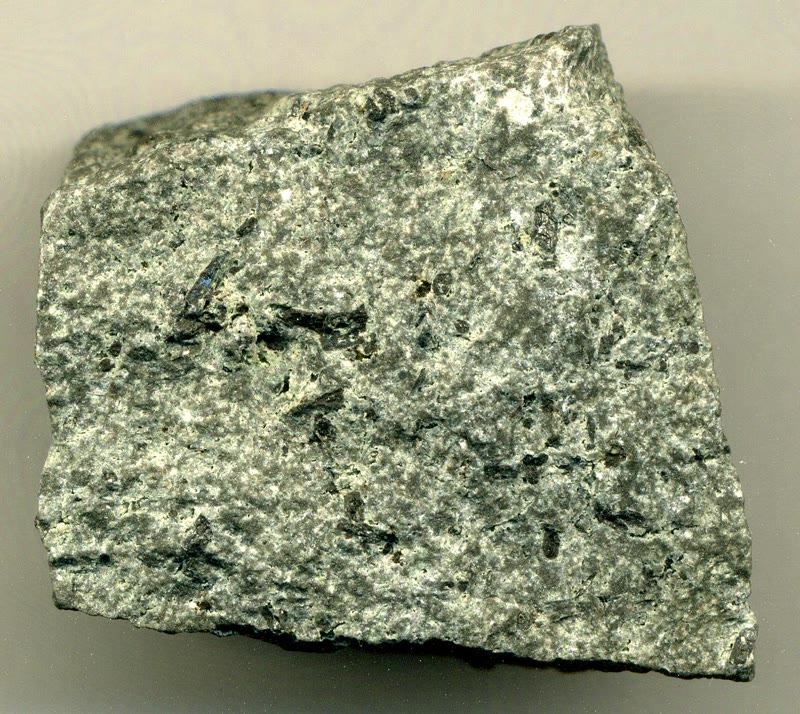
\includegraphics[height=4.4cm]{images/book2/g12-stjohn-andesite.jpg}\hspace{0.03\linewidth}%
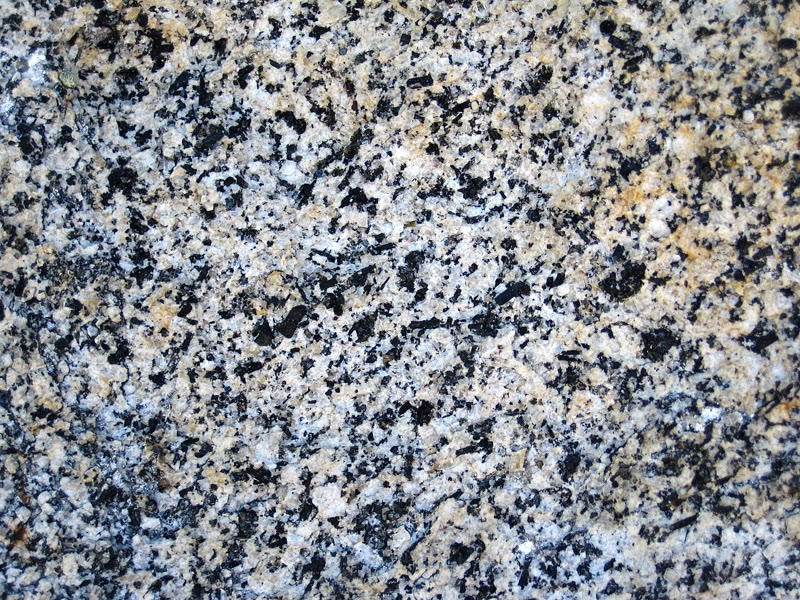
\includegraphics[height=4.4cm]{images/book2/g12-stjohn-granodiorite.jpg}

{\small Links: \omterm{def:g11:igneous-rocks:rock-names}{andesiet}, een fijnkorrelig \omterm{def:g11:igneous-rocks:volcanic-plutonic}{vulkanisch gesteente} van bogen. Rechts:
\omterm{def:g12:subduction-magmatism:granodiorite}{granodioriet} van de Sierra Nevada, met wit plagioklaas, grijs kwarts en
zwart biotiet en hoornblende. Foto's James St.~John (CC~BY~2.0).}
\end{omfigure}
% ledger: photo:g12-andesite, photo:g12-granodiorite

Gemiddeld bevat de bovenste \omterm{def:g12:continental-crust:continental-crust}{continentale korst} ongeveer \qty{67}{\percent}
\ce{SiO2}: ze is \omterm{def:g11:igneous-rocks:felsic-mafic}{felsisch}, zoals de granieten die bogen in grote hoeveelheden maken in
hun \omterm{def:g12:subduction-magmatism:batholith}{batholieten}.
% ledger: rg14:crust (upper crust SiO2 66.6 wt %), tulane:magma-types, tulane:intrusions

\begin{definition}[Batholiet]\label{def:g12:subduction-magmatism:batholith}
Een \emph{batholiet}\index{batholiet} is een grote massa \omterm{def:g11:igneous-rocks:volcanic-plutonic}{plutonisch gesteente} die
meer dan \qty{100}{km^2} beslaat waar erosie haar heeft blootgelegd. Ze ontstaat waar veel
\omterm{def:g11:igneous-rocks:intrusion}{plutonen}, de ene na de andere binnengedrongen, onder het oppervlak samenkomen.
\end{definition}
% ledger: earle:batholith, tulane:intrusions

Een van de grootste ter wereld, het Coast Plutonic Complex, loopt langs
de kust van de Stille Oceaan van de streek van Vancouver in het westen van Canada tot het
zuidoosten van Alaska. De \omterm{def:g12:subduction-magmatism:batholith}{batholiet} van de Sierra Nevada in Californië ontstond boven een
\omterm{def:g11:subduction-zones:subduction}{subductiezone}; de meeste van zijn granieten in Yosemite kristalliseerden in het
Krijt, 105 tot 85 miljoen jaar geleden. De gesteenten erboven werden over miljoenen jaren
afgesleten, en de \omterm{def:g11:igneous-rocks:intrusion}{plutonen} die diep beneden afkoelden, vormen nu
de bergen.
% ledger: earle:batholith, nps:yosemite, photo:g12-sierra-nevada (St. John description), ics:base.Cretaceous

\begin{omfigure}
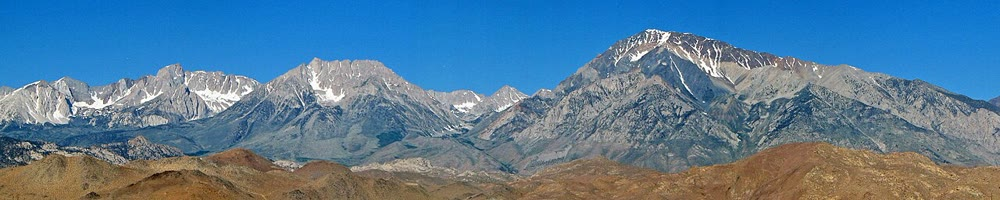
\includegraphics[width=0.94\linewidth]{images/book2/g12-stjohn-sierra-nevada-batholith.jpg}

{\small De Sierra Nevada, gezien vanuit het oosten: graniet en \omterm{def:g12:subduction-magmatism:granodiorite}{granodioriet} van
de \omterm{def:g12:subduction-magmatism:batholith}{batholiet} van de Sierra Nevada, die diep beneden kristalliseerde boven een
\omterm{def:g11:subduction-zones:subduction}{subductiezone} in het Krijt. Foto James St.~John
(CC~BY~2.0).}
\end{omfigure}
% ledger: photo:g12-sierra-nevada, nps:yosemite

\section{Hoe continenten groeien}

\begin{definition}[Continentale groei]\label{def:g12:subduction-magmatism:continental-growth}
\emph{Continentale groei}\index{continentale groei} is de toevoeging van nieuwe
\omterm{def:g12:continental-crust:continental-crust}{continentale korst}, gemaakt uit de mantel, vooral door het magmatisme van bogen.
De nettogroei van de continenten is die toevoeging min de \omterm{def:g12:continental-crust:continental-crust}{continentale korst}
die naar de mantel terugkeert.
\end{definition}
% ledger: sv09:growth, ss09:balance

Bogen zijn de plaats waar het lichte gesteente van de continenten wordt gemaakt. Schattingen van het
magma dat bogen vandaag toevoegen, zijn ongeveer \qty{1.5}{km^3} per jaar bij eilandbogen
en \qty{1.0}{km^3} per jaar bij continentale bogen; gemiddeld over de lange termijn
ongeveer \qty{2.7}{km^3} per jaar. Maar \omterm{def:g11:subduction-zones:subduction}{subductiezones} voeren ook \omterm{def:g12:continental-crust:continental-crust}{continentale
korst} terug naar de mantel: sediment dat met de \omterm{def:g11:subduction-zones:slab}{slab} mee omlaag gaat en stukken
van de bovenliggende plaat die er van onderen af worden geschraapt, ongeveer \qty{3.2}{km^3} per jaar.
De twee liggen dicht bij elkaar, en de nettogroei van de continenten over de laatste
paar honderd miljoen jaar kan nul zijn geweest, of zelfs negatief.
% ledger: sv09:growth, ss09:balance

Continenten groeien aan hun randen ook op een andere manier. \omterm{def:g12:continental-crust:continental-crust}{Continentale korst} is te
licht om te worden gesubduceerd, dus wanneer een plaat een continent in een trog voert, worden de
twee continenten bij een botsing aan elkaar gelast
(\cref{ch:g12:mountain-building}). Elk continent heeft een oude kern, een \omterm{def:g12:continental-crust:craton}{kraton},
omringd door gordels van jonger gesteente, de vervormde \omterm{def:g12:continental-crust:root}{wortels} van vroegere
gebergtegordels, die de ene na de andere aan zijn randen zijn toegevoegd
(\cref{ch:g12:continental-crust}).
% ledger: tulane:no-subduct (continental crust too buoyant to subduct), earle:collision, tulane:cratons

\section{Oefeningen}

\begin{exercise}[$\star$]\label{exo:g12:subduction-magmatism:1}
Geef het woord: (a) een rij vulkanen evenwijdig aan een trog, op de plaat
die niet zinkt; (b) smelten veroorzaakt door water aan een gesteente toe te voegen; (c) een
\omterm{def:g11:igneous-rocks:volcanic-plutonic}{plutonisch gesteente} met meer plagioklaas dan kaliveldspaat en meer dan
\qty{20}{\percent} kwarts; (d) een massa \omterm{def:g11:igneous-rocks:volcanic-plutonic}{plutonisch gesteente} groter dan
\qty{100}{km^2}; (e) de toevoeging van nieuwe \omterm{def:g12:continental-crust:continental-crust}{continentale korst} gemaakt uit de
mantel.
\end{exercise}

\begin{exercise}[$\star$]\label{exo:g12:subduction-magmatism:2}
Op 18 mei 1980 steeg de aszuil van de Mount St.~Helens meer dan \qty{24}{km}
in minder dan 15 minuten. (1) Wat was haar kleinste gemiddelde stijgsnelheid, in
\unit{km/h} en in \unit{m/s}? (2) Vergelijk die met de snelheid van de zijdelingse
explosie, minstens \qty{480}{km/h}.
\end{exercise}

\begin{exercise}[$\star$]\label{exo:g12:subduction-magmatism:3}
Van de 1214 vulkanen uit de catalogus die sinds het einde van de laatste
ijstijd actief zijn, staan er 838 boven een \omterm{def:g11:subduction-zones:subduction}{subductiezone}. (1) Welk percentage is dat? (2) Aan
welke kant van een trog staan deze vulkanen? (3) Waarom zijn er geen tussen
de trog en het vulkanische front?
\end{exercise}

\begin{exercise}[$\star$]\label{exo:g12:subduction-magmatism:4}
Een grofkorrelig gesteente bevat \qty{25}{\percent} kwarts, \qty{45}{\percent}
plagioklaas, \qty{15}{\percent} kaliveldspaat en \qty{15}{\percent}
biotiet en hoornblende. (1) Welk deel van zijn veldspaat is plagioklaas?
(2) Is het een \omterm{def:g12:subduction-magmatism:granodiorite}{granodioriet}?
\end{exercise}

\begin{exercise}[$\star$]\label{exo:g12:subduction-magmatism:5}
Geef twee redenen waarom de vulkanen van bogen explosiever uitbarsten dan die
van ruggen.
\end{exercise}

\begin{exercise}[$\star\star$]\label{exo:g12:subduction-magmatism:6}
(1) Een vulkanisch front ligt \qty{150}{km} van zijn trog, boven een \omterm{def:g11:subduction-zones:slab}{slab} die
\ang{35} helt. Hoe diep ligt de \omterm{def:g11:subduction-zones:slab}{slab} eronder? (2) Vergelijk met het
gemiddelde van \qty{105}{km}.
\end{exercise}

\begin{exercise}[$\star\star$]\label{exo:g12:subduction-magmatism:7}
Neem aan dat de \omterm{def:g11:subduction-zones:slab}{slab} onder elk vulkanisch front \qty{105}{km} diep ligt. Hoe ver van
de trog ligt het front wanneer de \omterm{def:g11:subduction-zones:slab}{slab} \ang{20} helt, en wanneer hij
\ang{45} helt? Wat zegt dat over waar je de boog moet zoeken?
\end{exercise}

\begin{exercise}[$\star\star$]\label{exo:g12:subduction-magmatism:8}
Op \qty{100}{km} is de druk ongeveer \qty{3.16}{GPa}. (1) Bereken met $T =
-5.104P^2 + 132.9P + 1120.7$ ($P$ in \unit{GPa}, $T$ in \unit{\celsius})
de temperatuur waarbij droge \omterm{def:g11:ocean-ridges:peridotite}{peridotiet} daar begint te smelten.
(2) Met water begint ze te smelten bij ongeveer \qty{1000}{\celsius}. Met hoeveel
verlaagt water die? (3) De mantelwig is daar, zeg,
\qty{1300}{\celsius}. Smelt hij droog? Nat?
\end{exercise}

\begin{exercise}[$\star\star$]\label{exo:g12:subduction-magmatism:9}
De puinlawine van de Mount St.~Helens verplaatste ongeveer \qty{2.5}{km^3}
gesteente. Bogen voegen ongeveer \qty{2.7}{km^3} nieuwe korst per jaar toe. (1) Hoeveel dagen
van het boogmagmatisme van de hele wereld vertegenwoordigt de lawine? (2) Waarom is de
vergelijking alleen een kwestie van grootte?
\end{exercise}

\begin{exercise}[$\star\star$]\label{exo:g12:subduction-magmatism:10}
(1) Hoeveel nieuwe korst voegen bogen in een miljoen jaar toe bij \qty{2.7}{km^3} per
jaar? (2) De \omterm{def:g12:continental-crust:continental-crust}{continentale korst} bevat ongeveer \qty{9e9}{km^3}. Hoe lang zouden
bogen alleen erover doen om dat volume te maken, als er niets van verloren ging? (3) Vergelijk met
de ouderdom van de Aarde, 4.5 miljard jaar.
\end{exercise}

\begin{exercise}[$\star\star$]\label{exo:g12:subduction-magmatism:11}
(1) Waarom worden in de doorsnede door Japan veel aardbevingen die ondieper zijn dan
\qty{70}{km} weggelaten wanneer de \omterm{def:g11:subduction-zones:slab}{slab} wordt aangepast? (2) De diepe aardbevingen liggen
op \qty{116}{km} diepte bij \ang{140.5}~OL en op \qty{80}{km} bij \ang{141.5}~OL, met
\qty{86.4}{km} per graad. Bereken de helling van de \omterm{def:g11:subduction-zones:slab}{slab}.
\end{exercise}

\begin{exercise}[$\star\star\star$]\label{exo:g12:subduction-magmatism:12}
Toon aan dat, voor een front op afstand $d$ van de trog boven een \omterm{def:g11:subduction-zones:slab}{slab} met helling
$\theta$, de afstand die langs de \omterm{def:g11:subduction-zones:slab}{slab} wordt gemeten van de trog tot het punt
onder het front $d/\cos\theta$ is. Hoe lang is die voor Japan ($d = \qty{270}{km}$,
$\theta = \ang{20}$)? De Pacifische plaat beweegt met ongeveer \qty{83}{mm} per jaar naar
Japan toe; hoe lang doet een stuk zeebodem er, als je die snelheid langs de hele \omterm{def:g11:subduction-zones:slab}{slab} aanneemt, over om van de trog tot onder de
vulkanen te reizen?
\end{exercise}
% ledger: usgs:tohoku (83 mm/yr)

\begin{exercise}[$\star\star\star$]\label{exo:g12:subduction-magmatism:13}
De magmakamer van de Mount St.~Helens is ongeveer \qty{1}{km} breed en loopt
van ongeveer 6 tot \qty{14}{km} diepte. (1) Schat haar volume door haar als een verticale cilinder
te behandelen. (2) Vergelijk het met de \qty{2.5}{km^3} van de lawine.
(3) Bereken de \omterm{def:g12:metamorphic-rocks:lithostatic}{lithostatische druk} aan haar boven- en onderkant ($\rho =
\qty{2830}{kg/m^3}$, $g = \qty{9.81}{m/s^2}$).
\end{exercise}

\begin{exercise}[$\star\star\star$]\label{exo:g12:subduction-magmatism:14}
Bogen voegen ongeveer \qty{2.7}{km^3} korst per jaar toe, en \omterm{def:g11:subduction-zones:subduction}{subductiezones} nemen er
ongeveer \qty{3.2}{km^3} terug. (1) Wat is de nettoverandering per miljoen jaar?
(2) Welk deel van een korst van \qty{9e9}{km^3} is dat over 500 miljoen jaar?
(3) De auteurs noemen de nettogroei ``feitelijk nul''. Waarom, gezien
de onzekerheid van elke schatting?
\end{exercise}

\begin{exercise}[$\star\star\star$]\label{exo:g12:subduction-magmatism:15}
Een \omterm{def:g12:subduction-magmatism:batholith}{batholiet} legt \qty{20000}{km^2} \omterm{def:g12:subduction-magmatism:granodiorite}{granodioriet} bloot waarvan de \omterm{def:g11:igneous-rocks:intrusion}{plutonen}
tussen 5 en \qty{15}{km} diepte zijn gestold. (1) Schat het volume magma
dat hij vertegenwoordigt, als je hem \qty{10}{km} dik neemt. (2) Bij \qty{1}{km^3} per jaar,
het tempo van alle continentale bogen van de wereld samen, hoe lang zouden die erover
doen om hem te maken? Wat zegt dat over de tijd waarin een
\omterm{def:g12:subduction-magmatism:batholith}{batholiet} wordt opgebouwd?
(3) Hoeveel gesteente moest er van erboven worden weggeërodeerd voordat hij te zien was?
\end{exercise}

\begin{problem}[{Weekendprobleem --- onder de vulkanen van Japan}]
\label{pb:g12:subduction-magmatism:1}
% ledger: data:b2-usgs-ne-japan, data:gvp, data:pb2002, sa06:slab-depth, hirschmann:solidus, wang20:wet-solidus, earle:arc-water, data:prem
% values (arc_magmatism.py): Megata 139.725, Iwate 141.001, trench 144.12; bins 140.5/141/141.5: 116.4/98.15/80.35 km; P_100km 3.157, dry_T_100km 1489
De vulkanen van het noordoosten van Japan tussen \ang{37.5} en \ang{40.5}~NB liggen
tussen \ang{139.7}~OL (Megata, de westelijkste) en \ang{141.0}~OL (Iwate, de
oostelijkste); de Japantrog ligt op \ang{144.1}~OL. De tabel geeft de
mediane diepte van de aardbevingen dieper dan \qty{70}{km} in drie stroken
lengte, 1976--2025. Neem \qty{111.2}{km} voor één breedtegraad.

\begin{center}
\small
\begin{tabular}{|l|c|c|c|}
\hline
lengte (\unit{\degree}~OL) & 140.5 & 141.0 & 141.5 \\ \hline
mediane diepte (\unit{km}) & 116 & 98 & 80 \\ \hline
\end{tabular}
\end{center}

\medskip
\noindent\textbf{Deel I --- Het vulkanische front.}
\begin{enumerate}
  \item Toon aan dat één lengtegraad op \ang{39}~NB ongeveer
        \qty{86.4}{km} is.
  \item Hoe ver ligt het vulkanische front van de trog?
  \item Hoe breed is de boog, van Iwate tot Megata?
  \item Op welke plaat staan de vulkanen, en aan welke kant van de
        trog?
  \item Waarom zijn er geen vulkanen tussen de trog en Iwate?
\end{enumerate}

\medskip
\noindent\textbf{Deel II --- De aardbevingsdoorsnede.}
\begin{enumerate}[resume]
  \item Met hoeveel kilometer veranderen de mediane diepten van
        \ang{140.5} tot \ang{141.5}~OL?
  \item Over welke horizontale afstand?
  \item Bereken de helling van de \omterm{def:g11:subduction-zones:slab}{slab}.
  \item Trek de lijn vanaf \ang{141.0}~OL, \qty{98}{km}, door tot aan het
        oppervlak. Waar bereikt ze dat, en hoe ver is dat van de trog?
  \item Opper waarom de \omterm{def:g11:subduction-zones:slab}{slab} dicht bij de trog minder steil is dan dieper.
\end{enumerate}

\medskip
\noindent\textbf{Deel III --- De slab onder de vulkanen.}
\begin{enumerate}[resume]
  \item Bereken $H = d\tan\theta$ met de afstand van vraag 2 en een helling
        van \ang{20}.
  \item Vergelijk die met de mediane diepte onder het front.
  \item Vergelijk beide met het bereik voor de wereld, 72 tot \qty{173}{km}, en het gemiddelde,
        \qty{105}{km}.
  \item Hoe diep ligt de \omterm{def:g11:subduction-zones:slab}{slab} onder Megata, volgens de lijn van vraag 9?
  \item Als je de korst van de boog ongeveer \qty{35}{km} dik neemt, ligt de
        bovenkant van de \omterm{def:g11:subduction-zones:slab}{slab} onder het front dan in de korst of in de mantel? Hoe
        ver onder de basis van de korst ligt hij?
\end{enumerate}

\medskip
\noindent\textbf{Deel IV --- Waar het water vandaan komt.}
\begin{enumerate}[resume]
  \item Waar kwam het water van de \omterm{def:g11:subduction-zones:slab}{slab} in zijn gesteenten terecht, en in welk
        mineraal zit er veel van?
  \item Op \qty{100}{km} is de druk ongeveer \qty{3.16}{GPa}. Bereken daar de
        droge solidus met $T = -5.104P^2 + 132.9P + 1120.7$.
  \item Met water ligt de solidus tussen 950 en \qty{1000}{\celsius}.
        Met hoeveel verlaagt water hem?
  \item Waarom kan de koude \omterm{def:g11:subduction-zones:slab}{slab} zelf niet de bron van het magma zijn?
  \item Vat samen: hoe diep ligt de \omterm{def:g11:subduction-zones:slab}{slab} onder het vulkanische front van het noordoosten van
        Japan?
\end{enumerate}
\end{problem}
